\documentclass[%
  degree=master,%
  classlevel=open,%classified,% 
  mathfont=mathptmx,%
  dedication=false,%
  chapbib=true,%
  %finish=peerreview,%
  driver=pdftex]{buptthesis}

%% 自定义导言区
% 在这里添加你需要的宏包、自定义命令、环境等
% \usepackage{...}
% \DeclareMathOperator{\CT}{H}
% \DeclareMathOperator{\Cov}{Cov}
\def\BUPTThesis{\textsc{BUPT}\-\textsc{Thesis}}

% 在这里添加图片文件搜索目录
%\graphicspath{{../}}
\graphicspath{{figures/}{chapters/}}
%% 自定义导言区结束

%% 加载缩略语定义
% 
% 更新记录:
%   {$LastChangedBy$}
%   {$LastChangedRevision$}
%   {$LastChangedDate$}

% 涉密论文保密年限
\classdur{三年}
        
% 学号
\studentid{2011111735}

% 论文题目
\ctitle{Si基GaAs异变外延及Si基异变量子点的研究}

% 申请学位
\cdegree{工学硕士}

% 院系名称
\cdepartment{信息光子学与光通信研究院}

% 专业名称
\cmajor{电子科学与技术}

% 你的姓名
\cauthor{王一帆} 

% 你导师的姓名
\csupervisor{任晓敏}

% 日期自动生成,也可以取消注释下面一行,自行指定日期
\cdate{\CJKdigits{2013}年\CJKnumber{12}月}

% 中文摘要
\cabstract{%
  本文介绍北京邮电大学研究生学位论文~\LaTeX{}~模板的使用方法。%
  本模板基本符合北京邮电大学研究生院培养与学位办公室于~2004~年~1~月~6~%
  日颁布的《北京邮电大学关于研究生学位论文各式的统一要求》。%

  中、英文摘要位于声明的次页,摘要应简明表达学位论文的内容要点,体现研%
  究工作的核心思想。重点说明本项科研的目的和意义、研究方法、研究成果、%
  结论,注意突出具有创新性的成果和新见解的部分。%

  关键词是为文献标引工作而从论文中选取出来的、用以表示全文主题内容信息%
  的术语。关键词排列在摘要内容的左下方,具体关键词之间以均匀间隔分开排%
  列,无需其它符号。%
}

% 中文关键词,关键词之间用\kwsep分割
\ckeywords{\TeX \kwsep \LaTeX \kwsep CJK \kwsep 模板 \kwsep 排版 \kwsep论文}

% 英文摘要
\eabstract{%
  This article presents, the \LaTeX{} thesis template for doctor/master 
  thesis of Beijing University of Posts and Telecommunications, and briefly 
  introduces the usage. The template fulfills the corresponding format 
  requirements issused by academic administration of Beijing University of 
  Posts and Telecommunications Graduate School on January 6, 2004. 

  The Chinese and English abstract should appear after the declaration page. 
  The abstract should present the core of the research work, especially the 
  purpose and importance of the research, the method adopted, the results, 
  and the conclusion.

  Key words are terms selected for documentation indexing, which should 
  present the main contributions of the thesis. Key words are aligned at the 
  bottom left side of the abstract content. Key words should be seperated by 
  spaces but not any other symbols.
}

% 英文关键词,也用\kwsep分割
\ekeywords{%
  \TeX \kwsep \LaTeX \kwsep CJK \kwsep template \kwsep 
  typesetting \kwsep thesis}
%\makeatother

%%% Local Variables:
%%% mode: latex
%%% TeX-master: "bare_thesis"
%%% End:


\loadglsentries{acronyms}

%% 攻读学位期间发表论文
% 用 \newcite{<suffix>}{<caption>} 声明不同的论文类型(例如: 期刊论文、会议论文等)。每一个类型的对应的 .bib 文件用 \bibliography<suffix> 命令加载,用 \nocite<suffix> 命令引用。具体请参考 pubs.tex 中的示例
\newcite{jrnl}{期刊论文}
\newcite{conf}{会议论文}

\begin{document}
%% 声明前置部分
\makefrontmatter

%% 生成主要符号对照表
% 学位论文 : 符号说明
% 
% 更新记录:
%   {$LastChangedBy$}
%   {$LastChangedRevision$}
%   {$LastChangedDate$}

\begin{listofnotations}
\item [$(\cdot)^*$] 复共轭
\item [$(\cdot)^{\mathrm T}$] 矩阵转置
\item [$(\cdot)^{\mathrm H}$] 矩阵共轭转置
\item [$\boldsymbol{X}$] 矩阵或向量
\item [$\mathcal{A}$] 集合
\item [$\mathcal{A}\times\mathcal{B}$] 
  集合~$\mathcal{A}$~与集合~$\mathcal{B}$~的~Cartesian~积,
  即~$\mathcal{A}\times\mathcal{B}=\{(a,b):a\in\mathcal{A},b\in\mathcal{B}\}$
\end{listofnotations}

%%% Local Variables: 
%%% mode: latex
%%% TeX-master: "bare_thesis"
%%% End: 


%% 主体部分
\mainmatter
% 用\include{}命令引用各章.tex文件
% 学位论文 : 第一章  绪论
% 
% 更新记录:
%   {$LastChangedBy$}
%   {$LastChangedRevision$}
%   {$LastChangedDate$}

\chapter{绪论}

\section{研究背景}


随着社会的发展与科学技术的进步,人们对信息服务的需求量与日俱增,信息产业已经成为关系国计民生的支柱性产业。世界各国纷纷投入大量的资金、人力、物力,致力于发展本国的信息产业,美国“信息高速公路”,韩国“IT大运河”,欧盟“宽带战略”等等,信息产业已经成为体现一个国家综合国力的重要指标。为了适应全球信息产业革命的进程,《国家中长期科学和技术发展规划纲要》明确提出:到2020 年,我国要“掌握一批事关国家竞争力的装备制造业和信息产业核心技术,使制造业和信息产业技术水平进入世界先进行列。”作为现代信息技术的主要载体,光传输网络的发展在我国信息产业建设中起着举足轻重的作用。所以,光网络的发展就成为我国信息产业建设的首要任务。同时,这种战略上的重大需求也给人们带来了各种技术上的挑战。如何建设功能更强、可靠性更好,功耗及成本更低、体积更小、使用维护更方便的光通信网络,成为信息技术研究人员所关注的热点。

显然,为了实现以上研究目标,单纯地依靠网络层面的优化是远远不够的,基础器件层面的进展更能够带动光通信网络的重大发展。目前,光通信器件还大多是相互独立,依靠传统的技术手段将其连接,组合成光网络。为了进一步降低成本,减小器件体积,光电子集成(即光电子器件之间,光电子与微电子器件之间的集成)就成为光通信器件的大势所趋。我们知道,制备光电子器件(如激光器,探测器,放大器等等)的基本材料都是半导体材料,尤其是Ⅲ-Ⅴ族半导体材料,为了实现不同器件之间的集成,不同的半导体材料之间的异质兼容就成为一个重要的研究方向。目前,光电子器件主要是GaAs基与InP基器件,微电子器件则是以Si基为主,而且,Si基造价低廉,应用广泛,且对于1.3-1.6μm的通信波长范围,Si是透明的,所以, Si基与GaAs基器件的异质兼容,一方面对光电子集成具有重大意义,另一方面能够有效地降低器件的制作成本。

自1963年阿尔费洛夫和克罗默两位科学家提出了半导体双异质结构以来,光电子器件经过了将近半个世纪的发展,已经取得了丰硕的成果,为光通信产业的快速发展起到了不可替代的推动作用。然而,相对于目前已经发展成熟的Si基大规模集成电路而言,光电子器件的集成度还不可同日而语。因此,将Si与III-V族材料集成成为了长期以来一个重要的研究方向。


\section{技术难点}

\section{研究现状}
我来占个位置。\cite{BUPT_Thesis_Format_2004}


% 本章参考文献
\ifx\usechapbib\empty
\bibliographystyle{buptthesis}
\bibliography{bare_thesis}
\fi

%%% Local Variables: 
%%% mode: latex
%%% TeX-master: "bare_thesis"
%%% End: 

% 学位论文 : 第二章 实验技术及设备简介
% 
% 更新记录:
%   {$LastChangedBy$}
%   {$LastChangedRevision$}
%   {$LastChangedDate$}

\chapter{实验技术及设备简介}
\section{生长设备}
<这类设备是干嘛的>
金属有机物气相外延沉积

{\hei 金属有机化合物化学气相沉积}

金属有机化合物化学气相沉积简介

金属有机化合物化学气相沉积(MOCVD),参见图\ref{fig:mocvd},又称金属有机化合物气相外延(MOVPE)、有机金属化合物气相外延(OMVPE),他是利用金属有机化合物进行金属输运的一种气相外延生长技术。MOCVD适于生长薄层、超薄层,乃至超晶格、量子阱材料等低维结构,并且可以进行多片和大片的外延生长,易实现产业化。

MOCVD技术具有很多优点:
\begin{enumerate}[(1)]
\item 因为MOCVD可采用金属有机化合物(简称MO源)的种类很多,所以该方法具有制备多种化合物和多元固溶体的灵活性;
\item 生长外延层的各组分和掺杂剂都是以气态的方式通入反应室的,通过控制气态源的流量和通断时间可以控制外延层的组分、厚度、界面和掺杂浓度;
\item 通常情况下晶体生长速率与III族源的流量成正比,因此生长速率调节范围较广。
\end{enumerate}

MOCVD技术现已获得广泛应用,成为制备化合物半导体异质结、低维结构材料,以及生产化合物半导体光电子、微电子器件的重要方法。用MOCVD技术生产半导体激光器、发光管、太阳能电池和高频、高速电子器件等都已形成产业。
金属有机化合物化学气相沉积原理

\begin{figure}[h]
	\centering
	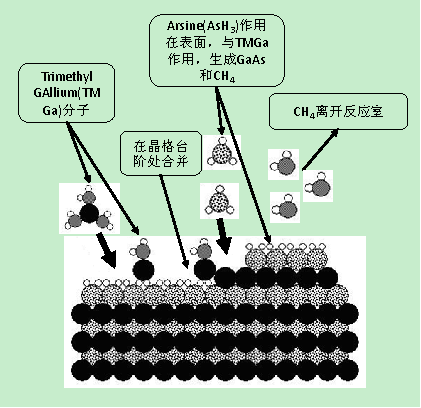
\includegraphics[width=0.8\textwidth]{ch02_MOCVD.pdf}
	\caption{MOCVD}
	\label{fig:mocvd}
\end{figure}

\section{表征设备}

<这类设备是干嘛的>

{\hei X-射线衍射仪} 这是一个我不知道是什么的设备,但听说它很有用,被用在了很多的领域,基本上实验室里的每一个实验都会用到这个设备,但它到底是做什么的呢,我是真的不知道,不过为了凑字我就只能写了这么长的一大串文字,总比粘一些不知道是啥的东西要好看多了。

{\hei 原子力显微镜}

{\hei 透射电镜}

{\hei 扫描电镜}

{\hei 腐蚀坑设备}

% 本章参考文献
\ifx\usechapbib\empty
\bibliographystyle{buptthesis}
\bibliography{../bare_thesis}
\fi

%%% Local Variables: 
%%% mode: latex
%%% TeX-master: "bare_thesis"
%%% End: 

% 学位论文 : 第三章 GaAs/Si异变外延两步法生长
% 
% 更新记录:
%   {$LastChangedBy$}
%   {$LastChangedRevision$}
%   {$LastChangedDate$}

\chapter{GaAs/Si异变外延两步法生长}

\section{GaAs/Si异变外延两步法生长,问题,目标}

GaAs与Si之间\%4的晶格失配对于在Si衬底上生长高质量GaAs外延片是最大的阻碍,Si衬底上最初的GaAs成核是生长过程中的关键步骤,并且在一定程度上决定着上面GaAs的质量。

晶片生长的成核有三种生长模式:层状生长(FM),岛状生长(VM)和SK模式生长,其中SK模式生长即是先岛状生长,接着是浸润层状生长。
前两种生长模式(FM和VM)可以用衬底表面能($ \gamma_{s}$)、外延层表面能($\gamma_{f}$)和两者之间的界面能($\gamma_{i}$)之间的关系来区分,如果衬底表面能远大于其他两者之和,则浸润机制发生,即是FM生长机制:

\begin{equation}
	\label{eq:FM}
 	\gamma_{s} > \gamma_{f} + \gamma_{i}
\end{equation}

若相反

\begin{equation}
	\label{eq:VM}
 	\gamma_{s} < \gamma_{f} + \gamma_{i}
\end{equation}

则无浸润发生,也就是VM生长机制。

对于SK生长模式,在开始生长阶段,表面能之间的关系是\ref{eq:FM},而在生长几个原子层之后表面能之间的关系则转换为\ref{eq:VM}。

GaAs/Si外延生长不包括浸润层,GaAs岛直接在Si衬底上形成,因此GaAs/Si最初的生长机制是VM。
Adomi 等阐述了衬底表面能的减少在GaAs/Si生长的过程中所起到的重要作用。他们在GaAs衬底上生长了0.9nm的Si薄膜(Si是赝形生长),然后再外延GaAs,则GaAs最初是岛状生长。以此推出,在Si表面用As或Ga钝化,减少其化学活性,有助于在最初的GaAs/Si外延生长过程中GaAs的岛状生长。从GaP/Si的生长中也可以推出该观点,GaP和Si的晶格失配很小,GaP/Si的最初生长也是岛状生长。


\begin{figure}[ht]
	\centering
	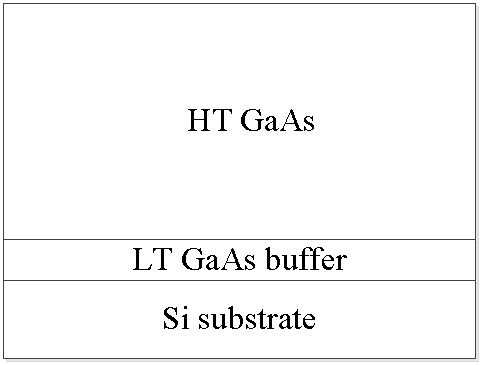
\includegraphics[width=0.8\textwidth]{ch03_TwoStepGrowth.pdf}
	\caption{TwoStep Growth}
	\label{fig:TwoStepGrowth}
\end{figure}

自从意识到用III族或V族元素钝化Si表面——在Si衬底上生长III-V族化合物的必要条件——导致了GaAs的最初生长是岛状生长,人们采取了许多不同的方法在Si衬底上沉积GaAs。包括:
使用外延衬底,例如先在Si衬底上沉积一层Si薄膜;低温生长最初的GaAs原子层;
用MEE外延方法分别外延Ga或As;生长无定形的Si或GaAs层。
到目前为止,应用最广泛的生长机制:两步法生长。
如图\ref{fig:TwoStepGrowth}所示,包括低温生长的GaAs缓冲层和最主要的高温生长的GaAs层。用这个生长顺序外延的原因是在结构位错产生之前低温生长的GaAs层是连续的。

\begin{figure}[ht]
	\centering
	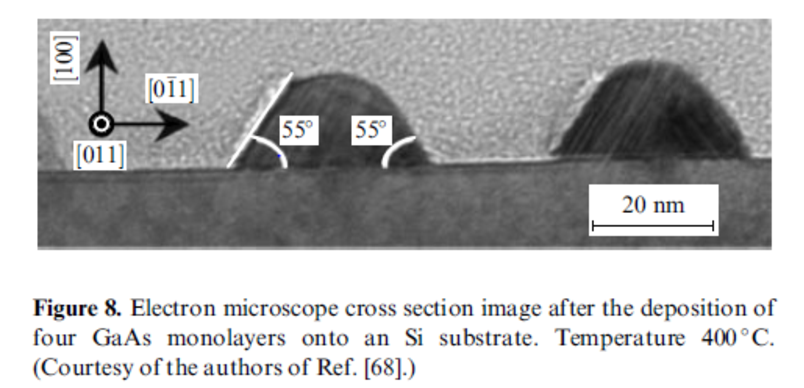
\includegraphics[width=0.8\textwidth]{ch03_GaAsIslands.pdf}
	\caption{GaAs Islands}
	\label{fig:GaAsIslands}
\end{figure}

在最初的生长阶段,GaAs岛的高度与横向宽度的比是1/2,而在Si衬底上生长的Ge的岛的高度与横向(\{105\}面)宽度的比是1/10。GaAs岛的高宽比远大于Ge岛,这表明Si基上GaAs成岛更加不可避免。图\ref{fig:GaAsIslands}是Si基上的GaAs岛的截面图。这些岛是在400℃的条件下沉积几个原子层的GaAs形成的,从图\ref{fig:GaAsIslands}中可以看出,这些岛是半球形的并且已经形成位错。

Si基上的GaAs岛可以看做是半球形,基于初期赝形生长的岛应力和形变计算,岛与衬底的界面是弯曲的,应力集中在岛的边缘,并且容易形成失配位错和其他的位错。
在1975年,Stowell详细地描述了在最初的薄膜沉积过程中,3D岛的合并导致了大量穿透位错的产生。
因此,人们需要研究在怎样的生长条件下失配位错能够产生在连续生长的薄膜中。


\begin{figure}[ht]
	\centering
	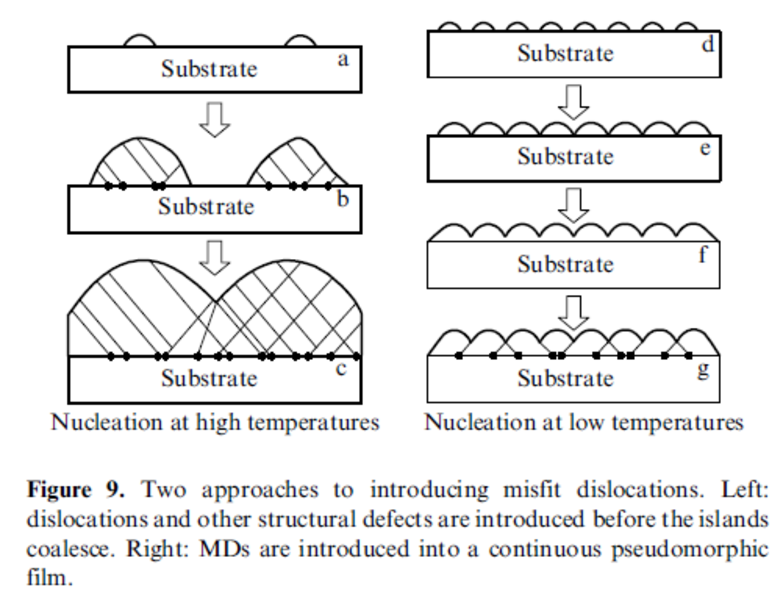
\includegraphics[width=0.8\textwidth]{ch03_IslandsGrowthProcedure.pdf}
	\caption{Islands Growth Procedure}
	\label{fig:IslandsGrowthProc}
\end{figure}

最初的生长温度越低,成岛的原子扩散区域越小,因此岛的密度就越大。图\ref{fig:IslandsGrowthProc}中是GaAs通过岛的合并形成层状的两种方式:一种是高温生长,另一种是低温生长。
以GaAs的生长温度为550℃-600℃为标准,当生长温度为400℃时,GaAs岛在合并之前就已经形成位错(图\ref{fig:IslandsGrowthProc}b),当这些岛开始合并时(图\ref{fig:IslandsGrowthProc}c),大量移动位错产生,这些位错用退火、高温生长厚外延层等方法都很难消除。

如果赝型生长的GaAs岛的合并方式如图 \ref{fig:IslandsGrowthProc}e和图\ref{fig:IslandsGrowthProc}f,粗糙的表面会产生很多位错,
这些位错会引入到连续生长的GaAs薄膜中(图\ref{fig:IslandsGrowthProc}g)。
因为低温生长的岛的密度比高温生长的岛的密度至少要高一个数量级,所以会导致表面形成的位错密度也较高(图\ref{fig:IslandsGrowthProc}f和图\ref{fig:IslandsGrowthProc}g)。
然而经实验表明,最初的GaAs薄膜用低温生长的GaAs外延层会降低XRD摇摆曲线的FWHM,表明提高了外延片的晶体质量。这应该怎么解释呢?一个可能的答案就是在GaAs合并时形成的失配位错变化较少,移动能力较强,所以在生长过程中,许多位错都能够消失。

据我们所知,到目前为止,对于初期的GaAs/Si的生长并没有详细的纳米级研究,因此不能直接观察到岛状生长到连续生长之间的变化。但是大量实验表明最初的GaAs用低温生长可以极大地改善GaAs外延层的晶体质量,但是这种生长方式的机制需要进一步的研究。


\section{衬底处理}

我们所使用的Si (001) 衬底是由天津通美公司提供的,偏角为偏向<011>4°。

对于Si衬底,表面常常有O,C杂质污染,在空气中极容易形成Si-O键,而作为外延薄膜衬底,它必须是完整,清洁并具有特定晶向,其中$SiO_x$可在超高真空下加热至1000℃把它除掉,但对于C污染,去除比较困难,表面上的SiC小团对外延层又非常有害,因此,必须寻找化学方法对Si表面进行处理。由于Si-O键的键能(439kJ/mol)比较大,而Si-H键的键能(222kJ/mol)比较小,因此Si表面极易被氧化,形成的氧化膜很稳定,要打开Si-O键所需的温度高于1000℃,而打开Si-H键所需的温度低于800℃。而MOCVD生长的温控平台一般为电热石墨舟结构,温度不宜长时间过高(>900℃)。如果不能在生长前断开所有的Si-O键去氧化,GaAs原子就很难与Si表面原子成键,导致外延质量急剧下降,因此Si片的氢化是非常重要的一步,另外Si表面一般还会吸附C等杂质,必须进行化学清洗。

1.首先预处理Si衬底,包括清洗、氢化、甩干。

第一步,用丙酮进行超声清洗,去除表面油脂等有机物。第二步,在$H_2 SO_4:H_2 O_2=3:1$溶液里煮洗至$H_2 O_2$完全挥发冒白烟,去除大部分有机物。第三步,在$NH_3•OH:H_2 O_2:H_2 O=1:1:6$溶液中,加热至75℃~85℃10min(由于氨水对硅有腐蚀作用,所以时间不能太长),去除金属杂质。第四步,在$HCl:H_2 O_2:H_2 O=1:1:6$,加热至75℃~85℃,盐酸对硅无腐蚀作用,可加热使得$H_2 O_2$完全挥发,去除表面金属离子。第五步,用HF漂洗5-10s,去除表面氧化层。第六步,用甩干机甩干并置入手套箱,尽量减少Si衬底与空气的接触时间。

2.高温烘烤、As钝化

经预处理的Si衬底送入反应室后,升温至750℃烘烤15min,烘烤的目的是使Si-H键脱离,然后在此温度下通入$AH_3$钝化3min,目的是使生长时先形成Si-As键,它相比Si-Ga更易成键。如前所述,这样可以减少反相畴和进一步清洁Si表面,以便为下一步生长做准备。
基于低温缓冲层的GaAs/Si直接外延的基本生长条件为:

\begin{enumerate}[(1)]
	\item 反应室压力为100Torr;
	\item 石墨舟转速为100rpm;
	\item III族源和V族源的载气(H2)总流量为12L/min;
	\item 三区石墨加热器的Zone A/B/C Ratio分别设定为39\%、45\%和80\%;
\end{enumerate}




\section{分项优化}

\subsection{低温缓冲层温度的优化}

大量实验表明,最优的低温缓冲层的生长温度在400-450℃之间,当第一步低温GaAs的生长温度高于450℃时,第二步高温GaAs的表面将变得粗糙;当第一步低温GaAs的生长温度低于400℃时,GaAs沉积可能不会发生。因此我们对低温缓冲层的温度进行了优化。

\begin{table*}[htbp] 
	\centering
	\caption{\label{tab:test1}低温缓冲层温度的优化}  
	\begin{tabular}{m{.15\textwidth}<{\centering}m{.3\textwidth}<{\centering}m{.25\textwidth}<{\centering}}   
		\toprule
			Sample no. & LT buffer growth temperature(℃) & DCXRD FWHM (arcsec) \\
		\midrule 
			A1 & 450 & 470.9 \\
			A2 & 460 & 501.3 \\
			A3 & 440 & 462.2 \\
			A4 & 420 & 462.6 \\
		\bottomrule
	\end{tabular}
\end{table*}

这一系列的样品低温缓冲层的温度分别为460、450、440和420℃,其他生长条件都是完全一样的:高温层的生长温度为630℃,生长速率为        ,生长厚度为900nm,且这些样品的表面都是光亮的。上图给出了不同低温缓冲层的生长温度对于外延片XRD半高宽的影响,可以看出当低温缓冲层的温度为440℃和420℃时,测得的XRD半高宽基本相同(462arcsec),我们选取了420℃作为了后续低温缓冲层的生长温度。


\subsection{低温缓冲层厚度的优化}

\begin{table*}[htbp] 
	\centering
	\caption{\label{tab:test2}低温缓冲层厚度的优化}  
	\begin{tabular}{m{.1\textwidth}<{\centering}m{.3\textwidth}<{\centering}m{.2\textwidth}<{\centering}m{.25\textwidth}<{\centering}}   
		\toprule
			Sample no. & LT buffer growth time(s) & DCXRD FWHM (arcsec) & RMS roughness (nm) in 10μm×10μm \\
		\midrule
			A1 & 400 & 431.1 & 6.991 \\
			A2 & 600 & 412.9 & 3.641 \\
			A3 & 800 & 447.6 & 3.23 \\
		\bottomrule
	\end{tabular}
\end{table*}

当高温层生长温度和厚度固定(温度:685℃,厚度:900nm),低温缓冲层生长温度为420℃时,优化低温缓冲层的生长时间,即优化低温缓冲层的厚度。当低温缓冲层生长时间为600s(后经TEM测试,此时厚度为70nm)时,外延片的XRD半高宽最窄,晶体质量最好,所以选取低温缓冲层厚度70nm作为后续外延片生长的低温缓冲层厚度。


\subsection{低温缓冲层种类的优化}

仅仅依靠高温生长并不能满足整个异质结构对于GaAs/Si外延片的要求,当最初的生长层的厚度、掺杂浓度和掺杂类型不同的时候,接下来的生长温度就不能超过一个固定的限制。由于这个原因,人们在GaAs和Si衬底之间采用不同材料的低温缓冲层,

\begin{table*}[htbp] 
	\centering
	\caption{\label{tab:test3}低温缓冲层种类的优化}  
	\begin{tabular}{m{.1\textwidth}<{\centering}m{.3\textwidth}<{\centering}m{.2\textwidth}<{\centering}m{.25\textwidth}<{\centering}}   
		\toprule
			Sample no. & Growth procedure & DCXRD FWHM (arcsec) & RMS roughness (nm) in 10μm×10μm \\
		\midrule
			A1 & GaAs buffer layer & 412 & 3.6 \\
			A2 & AlAs buffer layer & 401 & 3.4 \\
			A3 & AlGaAs/GaAs buffer layer & 447 & 6.3 \\
		\bottomrule
	\end{tabular}
\end{table*}

在固定的低温缓冲层生长温度和厚度(温度:420℃,厚度:70nm)、固定的高温层生长温度和厚度(温度:685℃,厚度:900nm)下,当低温缓冲层为AlAs时,XRD半高宽最窄,晶体质量最好。但是由于Al易氧化,后续的生长没有采用AlAs缓冲层。

\section{结论}

% 本章参考文献
\ifx\usechapbib\empty
\bibliographystyle{buptthesis}
\bibliography{../bare_thesis}
\fi

%%% Local Variables: 
%%% mode: latex
%%% TeX-master: "bare_thesis"
%%% End: 

% 学位论文 : 第二章 实验技术及设备简介
% 
% 更新记录:
%   {$LastChangedBy$}
%   {$LastChangedRevision$}
%   {$LastChangedDate$}

\chapter{GaAs/Si异变外延三步法生长}
\section{三步法动机+存在的问题+所以我们优化了+我们对比了+可能可以做的更好+怎么做了+对比}

\section{三步法优化方法}

\section{两步法与三步法的比较}

\subsection{中间温度层温度的优化}

\subsection{插入循环退火}

\section{InGaAs/GaAs应变超晶格的优化}

\section{InGaAs/GaAs、AlGaAs/GaAs、GaAsP/GaAs应变超晶格的比较}

\section{结论}

三步法好处

三步法到头了,另选其他方案,量子点方案解决

% 本章参考文献
\ifx\usechapbib\empty
\bibliographystyle{buptthesis}
\bibliography{../bare_thesis}
\fi

%%% Local Variables: 
%%% mode: latex
%%% TeX-master: "bare_thesis"
%%% End: 

% 学位论文 : 第二章 实验技术及设备简介
% 
% 更新记录:
%   {$LastChangedBy$}
%   {$LastChangedRevision$}
%   {$LastChangedDate$}

\chapter{GaAs/Si异变外延插入量子点位错阻挡层}
\section{背景}
量子点,为啥能解决
方案概要,量子点⇒异变外延生长

\section{量子点生长}

\subsection{单层量子点的生长}

\subsection{多层量子点的生长}

\subsection{与GaAs基量子点对比}

\section{量子点做位错阻挡层的GaAs/Si异变外延生长}
我来占个位置。\cite{BUPT_Thesis_Format_2004}



% 本章参考文献
\ifx\usechapbib\empty
\bibliographystyle{buptthesis}
\bibliography{bare_thesis}
\fi

%%% Local Variables: 
%%% mode: latex
%%% TeX-master: "bare_thesis"
%%% End: 

% 学位论文 : 第一章  绪论
% 
% 更新记录:
%   {$LastChangedBy$}
%   {$LastChangedRevision$}
%   {$LastChangedDate$}

\chapter{绪论}
北京邮电大学\gls*{BUPT}研究生院培养与学位办公室于2004年1月6日颁布了《北
京邮电大学关于研究生学位论文格式的统一要求》(下简称“要
求”)\cite{BUPT_Thesis_Format_2004},对研究生学位论文的格式要求做出了文
字性的描述和说明。但是迄今为止,研究生院尚未发布统一的论文模板。对于已
经、正在或者即将撰写学位论文的同学都只能按照该要求的规定自行调整其学位
论文的格式,一方面给大家增加了繁重的排版工作,另一方面也不利于统一全校
的论文格式。

2007~年~9~月,北京邮电大学无线新技术研究所\gls*{WTI}的王旭博士制作并发
布了~latex-bupt \CJKemdash北京邮电大学博士毕业论文~\LaTeX~模板(非官方
版)\cite{latex-bupt}。该模板可以满足官方论文格式要
求\cite{BUPT_Thesis_Format_2004},但是在一些细节上的处理还有待改进,例
如:
\begin{itemize}
\item 参考文献不能分列在各章末尾;
\item 不能利用~BiBTeX~处理发表学术论文列表;
\item 参考文献的格式上赏不能完全满足学校要求等。
\end{itemize}

本模板在清华大学学位论文~\LaTeX~模板\cite{thuthesis}的基础
上,根据\onlinecite{BUPT_Thesis_Format_2004}的要求进行了改写,除符合具
备\onlinecite{BUPT_Thesis_Format_2004}的全部要求,还根据国家标准进行了
适当的扩充和完善。

\section{中文信息处理软件的国内外发展现状}
中文信息处理软件可以分为字处理软件和排版软件两大类。字处理软件包括以下
功能:字体、字号设定,英文断字,拼写和语法检查等。通常字处理软件处理文
档的规模比较小,一般是作为办公自动化套件的一个重要组成部分,目前广泛使
用的中文字处理软件主要包括微软~Office~套件中的~Word、金山公司的~WPS,以
及开源社区的~OpenOffice~等。排版软件则是针对大规模专业出版印刷而设计的
一类软件,其主要功能是文字图像定位,基本图形绘制等。排版软件相对于字处
理软件其专业针对性更强,目前广泛使用的中文排版软件主要包括北大方正的书
版系列软件,飞腾系列软件,蒙泰桌面出版系统,Adobe~公司的~PageMaker,
FrameMaker,以及~QuarkPress~公司的~PassPort~等。除此而
外,由~D.~E.~Knuth~编写的~\TeX~和由~L.~Lamport~编写的~\LaTeX~也是学术界
广泛的应用排版软件。

微软公司的~Word~是目前国内最为普及的字处理软件之一,也是大多数学校规定
的学位论文编辑排版工具。不容否认,Word~在简单文书(例如:通知、简报
等)编辑排版方面具有方便快捷的优势,而且其对多人协同编辑的支持也给文字
修订工作带来了极佳的用户体验。但是从实际使用的情况看,尽管~Word~已经经
历了第~12~个版本的改进,但是其对于处理大型文书文稿(例如:书籍、学位论
文等)的能力仍然有待进一步完善和提高。由于~Word~版本不兼容造成的来回反
复,也是使用~Word~编辑文字稿件的烦事之一。另外,由于~Word~对数学公式编
辑的支持一直延续其“对象链接与嵌入”(Object Linking and
Embedding,OLE)的设计理念,这也使得每位使用~Word~排版过理工类的文字资
料的人都有一段或多段刻骨铭心的痛苦经历,往往花在调整格式这种~dirty
work~上的时间和花在编写文章内容上的时间差不多或着甚至更多。

北大方正的书版系列软件是专业中文出版领域的权威,国内几乎所有的大型出版
社、报社、政府机关几乎都使用书版系列软件对其出版的书籍、报纸和公文进行
编辑排版。但是,书版软件作为方正电子出版流程中的一个主要组成部分,主要
定位于印前排版环节,面向专业排版工作人员。因此,学习和使用使用书版软件
需要花费较长的时间来熟悉复杂的排版命令,发排后需要使用专用的~RIP~软件或
者方正的专用打印机才能输出样张等。

美国~Stanford~大学的荣誉退休教授~D.~E.~Knuth~在~197x~年独自一人开发
了~\TeX~排版系统,随后,L.~Lamport~为~\TeX~编写了一系列的宏包使得~\TeX~的
使用更加方便,这些宏包被称为~\LaTeX。自从~\TeX/\LaTeX~问世以来它们就受
到了学术界的青睐,目前几乎所有的国外出版社都接受或指定使用~
\TeX/\LaTeX~对稿件进行排版编辑。19xx~年,中国科学院的张林波研究员开发
了~CCT~使得~\LaTeX~可以用于中文文稿的处理。德国的W.~Lemberg,编写
了~CJK~宏包为~\LaTeX~提供了中日韩三国语言的解决方案。使
用~\TeX/\LaTeX~排版学术论文的最大优势在于,它让作者可以不用为排版输出的
具体格式操心,而全心投入文章、书稿内容的编写上,最大程度的降低作者从事
排版~dirty work~的工作量。

目前,我国的清华大学、哈尔滨工业大学、西安电子科技大学、西安交通大学等
都已经纷纷制作了本校学位论文的~\LaTeX~模板,并接受使用~\LaTeX~排版的学
位论文。

\section{本说明的主要内容}
本说明全面介绍了如何使用~\BUPTThesis~来排版符
合\onlinecite{BUPT_Thesis_Format_2004}规定的北京邮电大学学位论文。全文
内容安排如下:

\begin{enumerate}
\item 第二章介绍……
\item ……
\end{enumerate}

\begin{figure}[h]
 \centering
 
\includegraphics[width=0.2\textwidth]{amss.eps}
 \caption{中科院数学与系统科学研究院院徽(在页面中间)}
 \label{fig:amss1}
\end{figure}

我来占个位置。\cite{BUPT_Thesis_Format_2004}

% 本章参考文献
\ifx\usechapbib\empty
\bibliographystyle{buptthesis}
\bibliography{bare_thesis}
\fi

%%% Local Variables: 
%%% mode: latex
%%% TeX-master: "bare_thesis"
%%% End: 


%% 附录部分

% 如果有两个或两个以上的附录, 使用appendix环境
\begin{appendix}
  \chapter{不定型($0/0$)极限的计算}
\begin{theorem}[L'Hospital法则]
  若
  \begin{enumerate}
  \item 当~$x \to a$~时,函数~$f(x)$~和~$g(x)$~都趋于零;
  \item 在点~$a$~某去心邻域内,$f'(x)$~和~$g'(x)$~都存在,且~$g'(x)
    \neq 0$;
  \item $\displaystyle\lim_{x \to a} \dfrac{f'(x)}{g'(x)}$~存在(或为无穷大),
  \end{enumerate}
  那么
  \begin{align}
    \label{eq:app:lhospital}
    \lim_{x \to a} \frac{f(x)}{g(x)} = \lim_{x \to a} \frac{f'(x)}{g'(x)}.
  \end{align}
\end{theorem}
\begin{proof}
  以下只证明两函数~$f(x)$~和~$g(x)$~在~$x = a$~为光滑函数的情形。由
  于~$f(a) = g(a) = 0$,原极限可以重写为
  \begin{align*}
    \lim_{x \to a} \frac{f(x) - f(a)}{g(x) - g(a)}.
  \end{align*}
  对分子分母同时除以~$(x - a)$,得到
  \begin{align*}
    \lim_{x \to a} \frac{%
      \dfrac{f(x) - f(a)}{x - a}
    }{%
      \dfrac{g(x) - g(a)}{x - a}
    } &
    = \frac{%
      \displaystyle\lim_{x \to a} \frac{f(x) - f(a)}{x - a}
    }{%
      \displaystyle\lim_{x \to a} \frac{g(x) - g(a)}{x - a}
    }.
  \end{align*}
  分子分母各得一差商极限,即函数~$f(x)$~和~$g(x)$~分别在~$x = a$~处的导
  数
  \begin{align*}
    \lim_{x \to a} \frac{f(x)}{g(x)} &
    = \frac{f'(a)}{g'(a)}.
  \end{align*}
  由光滑函数的导函数必为一光滑函数,故~\eqref{eq:app:lhospital}~得证。
\end{proof}

%%% Local Variables: 
%%% mode: latex
%%% TeX-master: "bare_thesis"
%%% End: 

  % 自动抽取生成缩略语表作为附录A
  \tableofacronyms
  % 用\input{}添加其他的附录
  % \input{...}
\end{appendix}

% 如果只有一个附录, 使用appendix*环境
% \begin{appendix*}
%   % 自动抽取生成缩略语表作为附录A
%   % \tableofacronyms
% \end{appendix*}

\ifx\usechapbib\undefined
\bibliographystyle{buptthesis}
\bibliography{bare_thesis}
\fi

\backmatter
%% 致谢
% 博士学位论文 : 致谢
% 
% 更新记录:
%   {$LastChangedBy$}
%   {$LastChangedRevision$}
%   {$LastChangedDate$}

\begin{acknowledgement}
  % 感谢所有你应该感谢的人
  感谢Donald Ervin Knuth.
\end{acknowledgement}

%%% Local Variables: 
%%% mode: latex
%%% TeX-master: "bare_thesis"
%%% End: 


%% 在读期间论文发表情况
% 发表论文列表

% 攻读学位期间发表论文列表用 tableofpublications 环境产生。需要
% 在 bare_thesis.tex 的导言区用 \newcite{<name>}{<caption>} 声明不同类
% 型的论文,具体见导言区说明。

\begin{tableofpublications}
  \bibliographyjrnl{pubs}
  \nocitejrnl{paper1}
  \nocitejrnl{paper4}

  \bibliographyconf{pubs}
  \nociteconf{paper2}
  \nociteconf{paper3}
\end{tableofpublications}

%%% Local Variables: 
%%% mode: latex
%%% TeX-master: "bare_thesis"
%%% End: 


\newpage
\end{document}

%%% Local Variables: 
%%% mode: latex
%%% TeX-master: t
%%% End: 
